\documentclass[12pt,twoside]{article}
\bibliographystyle{vancouver}
\usepackage{graphicx}

\newcommand{\reporttitle}{CSCE-585: Machine Learning Systems\\
Project Proposal: Visual M.L. System for Identifying and Minimizing Civilian Fatality in Urban War Zones}
\newcommand{\reportauthor}{
    Logan Nall (github.com/Clnall),\\
    Walter Pach (github.com/waltster), \\
    Vera Svensson (github.com/Lux-Vera)
}
\newcommand{\reporttype}{Project Proposal}
\newcommand{\cid}{your college-id number}

% include files that load packages and define macros
%%%%%%%%%%%%%%%%%%%%%%%%%%%%%%%%%%%%%%%%%
% University Assignment Title Page 
% LaTeX Template
% Version 1.0 (27/12/12)
%
% This template has been downloaded from:
% http://www.LaTeXTemplates.com
%
% Original author:
% WikiBooks (http://en.wikibooks.org/wiki/LaTeX/Title_Creation)
%
% License:
% CC BY-NC-SA 3.0 (http://creativecommons.org/licenses/by-nc-sa/3.0/)
% 
% Instructions for using this template:
% This title page is capable of being compiled as is. This is not useful for 
% including it in another document. To do this, you have two options: 
%
% 1) Copy/paste everything between \begin{document} and \end{document} 
% starting at \begin{titlepage} and paste this into another LaTeX file where you 
% want your title page.
% OR
% 2) Remove everything outside the \begin{titlepage} and \end{titlepage} and 
% move this file to the same directory as the LaTeX file you wish to add it to. 
% Then add \input{./title_page_1.tex} to your LaTeX file where you want your
% title page.
%
%----------------------------------------------------------------------------------------
%	PACKAGES AND OTHER DOCUMENT CONFIGURATIONS
%----------------------------------------------------------------------------------------
\usepackage{ifxetex}
\usepackage{textpos}
\usepackage[numbers]{natbib}
\usepackage{kpfonts}
\usepackage[a4paper,hmargin=2.8cm,vmargin=2.0cm,includeheadfoot]{geometry}
\usepackage{ifxetex}
\usepackage{stackengine}
\usepackage{tabularx,longtable,multirow,subfigure,caption}%hangcaption
\usepackage{fncylab} %formatting of labels
\usepackage{fancyhdr}
\usepackage{color}
\usepackage[tight,ugly]{units}
\usepackage{url}
\usepackage{float}
\usepackage[english]{babel}
\usepackage{amsmath}
\usepackage{graphicx}
\usepackage[colorinlistoftodos]{todonotes}
\usepackage{dsfont}
\usepackage{epstopdf} % automatically replace .eps with .pdf in graphics
\usepackage{natbib}
\usepackage{backref}
\usepackage{array}
\usepackage{latexsym}
\usepackage{etoolbox}

\usepackage{enumerate} % for numbering with [a)] format 



\ifxetex
\usepackage{fontspec}
\setmainfont[Scale=.8]{OpenDyslexic-Regular}
\else
\usepackage[pdftex,pagebackref,hypertexnames=false,colorlinks]{hyperref} % provide links in pdf
\hypersetup{pdftitle={},
  pdfsubject={}, 
  pdfauthor={\reportauthor},
  pdfkeywords={}, 
  pdfstartview=FitH,
  pdfpagemode={UseOutlines},% None, FullScreen, UseOutlines
  bookmarksnumbered=true, bookmarksopen=true, colorlinks,
    citecolor=black,%
    filecolor=black,%
    linkcolor=black,%
    urlcolor=black}
\usepackage[all]{hypcap}
\fi

\usepackage{tcolorbox}

% various theorems
\usepackage{ntheorem}
\theoremstyle{break}
\newtheorem{lemma}{Lemma}
\newtheorem{theorem}{Theorem}
\newtheorem{remark}{Remark}
\newtheorem{definition}{Definition}
\newtheorem{proof}{Proof}

% example-environment
\newenvironment{example}[1][]
{ 
\vspace{4mm}
\noindent\makebox[\linewidth]{\rule{\hsize}{1.5pt}}
\textbf{Example #1}\\
}
{ 
\noindent\newline\makebox[\linewidth]{\rule{\hsize}{1.0pt}}
}



%\renewcommand{\rmdefault}{pplx} % Palatino
% \renewcommand{\rmdefault}{put} % Utopia

\ifxetex
\else
\renewcommand*{\rmdefault}{bch} % Charter
\renewcommand*{\ttdefault}{cmtt} % Computer Modern Typewriter
%\renewcommand*{\rmdefault}{phv} % Helvetica
%\renewcommand*{\rmdefault}{iwona} % Avant Garde
\fi

\setlength{\parindent}{0em}  % indentation of paragraph

\setlength{\headheight}{14.5pt}
\pagestyle{fancy}
\fancyfoot[ER,OL]{\thepage}%Page no. in the left on
                                %odd pages and on right on even pages
\fancyfoot[OC,EC]{\sffamily }
\renewcommand{\headrulewidth}{0.1pt}
\renewcommand{\footrulewidth}{0.1pt}
\captionsetup{margin=10pt,font=small,labelfont=bf}


%--- chapter heading

\def\@makechapterhead#1{%
  \vspace*{10\p@}%
  {\parindent \z@ \raggedright %\sffamily
        %{\Large \MakeUppercase{\@chapapp} \space \thechapter}
        %\\
        %\hrulefill
        %\par\nobreak
        %\vskip 10\p@
    \interlinepenalty\@M
    \Huge \bfseries 
    \thechapter \space\space #1\par\nobreak
    \vskip 30\p@
  }}

%---chapter heading for \chapter*  
\def\@makeschapterhead#1{%
  \vspace*{10\p@}%
  {\parindent \z@ \raggedright
    \sffamily
    \interlinepenalty\@M
    \Huge \bfseries  
    #1\par\nobreak
    \vskip 30\p@
  }}
  



% %%%%%%%%%%%%% boxit
\def\Beginboxit
   {\par
    \vbox\bgroup
	   \hrule
	   \hbox\bgroup
		  \vrule \kern1.2pt %
		  \vbox\bgroup\kern1.2pt
   }

\def\Endboxit{%
			      \kern1.2pt
		       \egroup
		  \kern1.2pt\vrule
		\egroup
	   \hrule
	 \egroup
   }	

\newenvironment{boxit}{\Beginboxit}{\Endboxit}
\newenvironment{boxit*}{\Beginboxit\hbox to\hsize{}}{\Endboxit}



\allowdisplaybreaks

\makeatletter
\newcounter{elimination@steps}
\newcolumntype{R}[1]{>{\raggedleft\arraybackslash$}p{#1}<{$}}
\def\elimination@num@rights{}
\def\elimination@num@variables{}
\def\elimination@col@width{}
\newenvironment{elimination}[4][0]
{
    \setcounter{elimination@steps}{0}
    \def\elimination@num@rights{#1}
    \def\elimination@num@variables{#2}
    \def\elimination@col@width{#3}
    \renewcommand{\arraystretch}{#4}
    \start@align\@ne\st@rredtrue\m@ne
}
{
    \endalign
    \ignorespacesafterend
}
\newcommand{\eliminationstep}[2]
{
    \ifnum\value{elimination@steps}>0\leadsto\quad\fi
    \left[
        \ifnum\elimination@num@rights>0
            \begin{array}
            {@{}*{\elimination@num@variables}{R{\elimination@col@width}}
            |@{}*{\elimination@num@rights}{R{\elimination@col@width}}}
        \else
            \begin{array}
            {@{}*{\elimination@num@variables}{R{\elimination@col@width}}}
        \fi
            #1
        \end{array}
    \right]
    & 
    \begin{array}{l}
        #2
    \end{array}
    &%                                    moved second & here
    \addtocounter{elimination@steps}{1}
}
\makeatother

%% Fast macro for column vectors
\makeatletter  
\def\colvec#1{\expandafter\colvec@i#1,,,,,,,,,\@nil}
\def\colvec@i#1,#2,#3,#4,#5,#6,#7,#8,#9\@nil{% 
  \ifx$#2$ \begin{bmatrix}#1\end{bmatrix} \else
    \ifx$#3$ \begin{bmatrix}#1\\#2\end{bmatrix} \else
      \ifx$#4$ \begin{bmatrix}#1\\#2\\#3\end{bmatrix}\else
        \ifx$#5$ \begin{bmatrix}#1\\#2\\#3\\#4\end{bmatrix}\else
          \ifx$#6$ \begin{bmatrix}#1\\#2\\#3\\#4\\#5\end{bmatrix}\else
            \ifx$#7$ \begin{bmatrix}#1\\#2\\#3\\#4\\#5\\#6\end{bmatrix}\else
              \ifx$#8$ \begin{bmatrix}#1\\#2\\#3\\#4\\#5\\#6\\#7\end{bmatrix}\else
                 \PackageError{Column Vector}{The vector you tried to write is too big, use bmatrix instead}{Try using the bmatrix environment}
              \fi
            \fi
          \fi
        \fi
      \fi
    \fi
  \fi 
}  
\makeatother

\robustify{\colvec}

%%% Local Variables: 
%%% mode: latex
%%% TeX-master: "notes"
%%% End: 

 % various packages needed for maths etc.
% quick way of adding a figure
\newcommand{\fig}[3]{
 \begin{center}
 \scalebox{#3}{\includegraphics[#2]{#1}}
 \end{center}
}

%\newcommand*{\point}[1]{\vec{\mkern0mu#1}}
\newcommand{\ci}[0]{\perp\!\!\!\!\!\perp} % conditional independence
\newcommand{\point}[1]{{#1}} % points 
\renewcommand{\vec}[1]{{\boldsymbol{{#1}}}} % vector
\newcommand{\mat}[1]{{\boldsymbol{{#1}}}} % matrix
\newcommand{\R}[0]{\mathds{R}} % real numbers
\newcommand{\Z}[0]{\mathds{Z}} % integers
\newcommand{\N}[0]{\mathds{N}} % natural numbers
\newcommand{\nat}[0]{\mathds{N}} % natural numbers
\newcommand{\Q}[0]{\mathds{Q}} % rational numbers
\ifxetex
\newcommand{\C}[0]{\mathds{C}} % complex numbers
\else
\newcommand{\C}[0]{\mathds{C}} % complex numbers
\fi
\newcommand{\tr}[0]{\text{tr}} % trace
\renewcommand{\d}[0]{\mathrm{d}} % total derivative
\newcommand{\inv}{^{-1}} % inverse
\newcommand{\id}{\mathrm{id}} % identity mapping
\renewcommand{\dim}{\mathrm{dim}} % dimension
\newcommand{\rank}[0]{\mathrm{rk}} % rank
\newcommand{\determ}[1]{\mathrm{det}(#1)} % determinant
\newcommand{\scp}[2]{\langle #1 , #2 \rangle}
\newcommand{\kernel}[0]{\mathrm{ker}} % kernel/nullspace
\newcommand{\img}[0]{\mathrm{Im}} % image
\newcommand{\idx}[1]{{(#1)}}
\DeclareMathOperator*{\diag}{diag}
\newcommand{\E}{\mathds{E}} % expectation
\newcommand{\var}{\mathds{V}} % variance
\newcommand{\gauss}[2]{\mathcal{N}\big(#1,\,#2\big)} % gaussian distribution N(.,.)
\newcommand{\gaussx}[3]{\mathcal{N}\big(#1\,|\,#2,\,#3\big)} % gaussian distribution N(.|.,.)
\newcommand{\gaussBig}[2]{\mathcal{N}\left(#1,\,#2\right)} % see above, but with brackets that adjust to the height of the arguments
\newcommand{\gaussxBig}[3]{\mathcal{N}\left(#1\,|\,#2,\,#3\right)} % see above, but with brackets that adjust to the height of the arguments
\DeclareMathOperator{\cov}{Cov} % covariance (matrix) 
\ifxetex
\renewcommand{\T}[0]{^\top} % transpose
\else
\newcommand{\T}[0]{^\top}
\fi
% matrix determinant
\newcommand{\matdet}[1]{
\left|
\begin{matrix}
#1
\end{matrix}
\right|
}



%%% various color definitions
\definecolor{darkgreen}{rgb}{0,0.6,0}

\newcommand{\blue}[1]{{\color{blue}#1}}
\newcommand{\red}[1]{{\color{red}#1}}
\newcommand{\green}[1]{{\color{darkgreen}#1}}
\newcommand{\orange}[1]{{\color{orange}#1}}
\newcommand{\magenta}[1]{{\color{magenta}#1}}
\newcommand{\cyan}[1]{{\color{cyan}#1}}


% redefine emph
\renewcommand{\emph}[1]{\blue{\bf{#1}}}

% place a colored box around a character
\gdef\colchar#1#2{%
  \tikz[baseline]{%
  \node[anchor=base,inner sep=2pt,outer sep=0pt,fill = #2!20] {#1};
    }%
}%

 % short-hand notation and macros

%%%%%%%%%%%%%%%%%%%%%%%%%%%%

\begin{document}
% front page
% Last modification: 2016-09-29 (Marc Deisenroth)
\begin{titlepage}

\newcommand{\HRule}{\rule{\linewidth}{0.5mm}} % Defines a new command for the horizontal lines, change thickness here


%----------------------------------------------------------------------------------------
%	LOGO SECTION
%----------------------------------------------------------------------------------------


\includegraphics[width = 4cm]{./figures/usc}\\[0.5cm] 

\begin{center} % Center remainder of the page

%----------------------------------------------------------------------------------------
%	HEADING SECTIONS
%----------------------------------------------------------------------------------------
\textsc{\LARGE \reporttype}\\[1.5cm] 
\textsc{\Large University of South Carolina}\\[0.5cm] 
\textsc{\large Computer Science and Engineering}\\[0.5cm] 
%----------------------------------------------------------------------------------------
%	TITLE SECTION
%----------------------------------------------------------------------------------------

\HRule \\[0.4cm]
{ \large \bfseries \reporttitle}\\ % Title of your document
\HRule \\[1.5cm]
\end{center}
%----------------------------------------------------------------------------------------
%	AUTHOR SECTION
%----------------------------------------------------------------------------------------

%\begin{minipage}{0.4\hsize}
\begin{center} \large
\textbf{Authors:}\\
\vspace{0.25cm}
\reportauthor%~(ID: Your USC ID) % Your name
\end{center}
\vspace{2cm}
\makeatletter
\begin{center}
    \@date 
\end{center}

\vfill % Fill the rest of the page with whitespace



\makeatother


\end{titlepage}



\tableofcontents
\newpage

%%%%%%%%%%%%%%%%%%%%%%%%%%%% Main document
\section{Project Repository}
The repository for our team can be found at \href{https://github.com/waltster/CSCE-585}{https://github.com/waltster/CSCE-585}. This repository is used for collaborating, issue tracking, and updating/version control.\\

This proposal can be identified by the GitHub tag: \emph{ProjectProposal}.

\section{Problem \& Interest}
With the proliferation of automated systems deployment in firms and organizations around the world, there is a demand for automated systems that produce both efficient and cost-effective solutions to problems previously requiring human intervention. In recent years, the application of artificially intelligent systems has provided the solution for many organizations in the form of models and systems that are able to intelligently predict and respond to data. This introduces many concerns and opens the possibility for deployment in novel situations and sectors. The application of A.I. systems is not limited by industry but rather will impact markets uniformly as the technology continues to evolve. Firms are presented with the problem of keeping pace with changing market conditions, availability of relevant A.I. systems, and quality of A.I. models. As firms and organizations begin to adopt A.I. technology, competition that spurs further adoption will occur. This causes early concerns to be paramount in sectors that directly influence human life.\\

With the advancements made in object detection and its deployment at the edge, the military applications of A.I. systems have increased. The subject of our concern is the use of A.I. systems in automated or supervised targeting systems involved in the use or training of weapons systems. This includes both unmanned and manned, both unsupervised and supervised weapons systems. In order to preserve human life in this context while maintaining the cost-effectiveness and efficiency of these A.I.-enabled systems, we hope to outline both the necessity and the feasibility of introducing new control mechanisms in this environment.\\

In this project, our goal will be to develop an A.I. model that is enabled to differentiate between common civilian and military vehicles, including classifications such as land vehicles, airplanes, helicopters, and drones. The problem presented includes both the issue of accuracy when human analysts apply characterization to targeting, as well as the ability to audit the success of the system with a clearly defined confidence metric.\\

Given the conditions of the Russia-Ukraine war and the escalating international tensions, paired with the rapid deployment of developmental weapons, we find it of particular interest to develop a built-in capability to identify and avoid civilian casualty. 

\newpage
\section{Background Literature / Related Work}
There are documented cases where A.I. systems have been deployed alongside or to replace human operators, including in recent conflict \cite{dronesAI}. This is of particular interest for highlighting the increasing role that M.L. systems are playing in production-level application.\\

CNN stands for Convolutional Neural Network and in ``A Fast Military Object Recognition using Extreme Learning Approach on CNN'' researchers look at combining ELM standing for Extreme Learning Machine to make up for the pitfalls of CNN \cite{CNN}. The goal of this research is to maintain the accuracy of CNN but to alleviate its long training times, have a smaller resource need, and having comparable speed as needed for field use. Previous works with CNN and ELM have been done in the past achieving an accuracy of close to 95\% albeit with long processing time and great commitment of resources while being trained. Data collected during the training time showed that CNN and ELM saved roughly 20\% on training time however utilizing more CPU and RAM. The outcome of needing more resources was predictable as compared to just running CNN; the researchers found that it would take an additional 79\% more resources, particularly for the CPU, for running models from both ELM and CNN. What researchers would come to conclude from using the two is the benefit of maintaining accuracy. In the test with CNN and CNN together with ELM, the pair had a 1\% higher accuracy while just CNN had 3\% greater results in the normal model test data. Through the five testing iteration CNN and ELM would achieve .86 accuracy while CNN .89 showing that 3\% difference.\\

Contrasting CNN and ELM individually, CNN would continue to produce better results in more complicated identifications such as helicopters over the single layer using ELM. But the need to combine the two stems from CNN's back-propagation leaving more to be desired in time saving capabilities.\cite{CNN}\\

\newpage
\begin{figure} [!h]
    \centering
    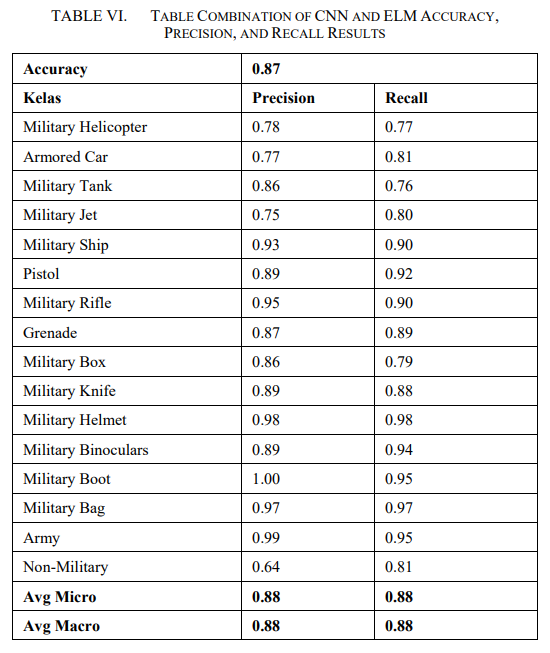
\includegraphics[width = \textwidth]{figures/precisionTable.png}
    \caption{CNN and ELM's Results \cite{CNN}}
    \label{fig:precisionTable}
\end{figure}

Information is vital to formulating decisions and the military has to make many decisions from the repetitive to the new. Machines can handle large data spectacularly well. In the paper ``Human-AI Cooperation to Benefit Military Decision Making'' authored by Karel van den Bosch and Adelbert Bronkhorst, they speak to the problem of bound rationality as Herbert Simon would refer to it where people are ``limited in their cognitive processing abilities when they have to deal with complex problems'' despite however rational they may be. Machine learning is already implemented and being improved to be able to suggest solutions. Allowing less time wasted sorting through data and more time utilized on developing the best solution. \\

From technology developing, drones are the latest to be introduced to the battlefield. Often used for surveillance, they have classification mainly that of weigh, payload, and range.\\

Class 1 and 2 are capable of having weapons because of their size and capable range. Class 3, 4, and 5 for closer range surveillance. Being able to identify civilian vehicles is not only important for drones but also for satellites. These methods of getting visual confirmation are the most frequently used. \\


A methodology for detecting military objects instead of civilian objects is the proposition for a multi-level CapsNet architecture \cite{objectDetect}. The idea of this method is to have an image go through the following:
\begin{enumerate}
    \itemsep0em 
    \item Convolutional Layer
    \item Primary Capsule Layer
    \item Class Capsule Layer
    \item Softmax Layer
\end{enumerate}
Then, having an output as a result of crossing through all the layers. The Convolutional Layer can be multiple layers as the input image is being scanned for features by the application of kernels. An interesting idea to keep account of is if the image is not black and white as in such an instance then the kernels used need to be 3D arrays to factor in depth juxtaposition to black and white's 2D kernels. The output from the Convolutional Layer goes into the Primary Capsule Layer that will formulate an array of feature maps to be reshape into a number of vectors by a dimension. An important step here is managing the vectors to be between 1 and 0 since probability will be used to determine object's presence, this step being called the "squash function". Class Capsule Layer is quite complicated where features for identification and classification will become the output. This is done through the process of route by agreement which seems to be a division of the output of the Primary Capsule Layer being contrasted against each other in three groups for a smaller output. This output is what the Softmax Layer ultimately weighs against each possible military object class providing the result. \cite{objectDetect}

\section{Data}
The M.L. system will be developed iteratively along the same methodology as the source. We plan on training our model on several different data sets to be able to evaluate how well it performs. Our model will begin being trained on a simple data set of different car makes and models. We plan to use the CompCars data set which is a data set from 2015 containing labeled images of cars.\cite{compCars} This data set is slightly lacking, since we want out model to be able to identify more than just cars. However, we think that it would be of interest to able to evaluate how well the model can differentiate between similar vehicles. Additionally, this will allow our boilerplate code to be developed iteratively and identify the libraries that we need to incorporate. \\

After our system has been adapted and trained on the sample car data, we will use a collection of military and civilian vehicles. We plan on using the ``Military and Civilian Vehicles Classification'' data set, available as FOSS \cite{militaryData}. It contains 6772 images of both civilian and military vehicles of different sorts. This will provide both the labelling and the images to train our final model. \\

As we continue the development of our model we might discover faults with these data sets, or find other data sets of interest. We are open to add, or switch, data sets along the way if we find it fitting.

\section{Methodology \& Integrations}
\subsection{Technological Methodology}
Our initial evaluation of the technology available suggests that our M.L. system will require many components to achieve full functionality. For the modelling and data representation, the best solution for our problem statement appears to be an object-detection model trained specifically to detect the presence of vehicles. This model will then be re-trained on another labelled data set with the nuance of military/civilian differences.\\

Our initial idea of the system is using static images that are fed through the object-detection model and outputs a classification with a confidence metric. We will achieve this through training a TensorFlow model. Our second iteration will be to use a video feed that is split into its static frames when movement occurs, with the same modelling process taking place.

\subsection{Developmental Methodology}
Our team's development methodology begins with a concern for the ease of delivery and adaptation of the A.I. model(s) and supporting infrastructure over time. This means that the process for both building, collaborating, and testing code must be able to scale appropriate to the needs, and that the system must function similarly as the scale of the deployment increases. We incorporate an iterative methodology, where each iteration produces an increase in accuracy, efficiency, or reliability.\\

\begin{center}
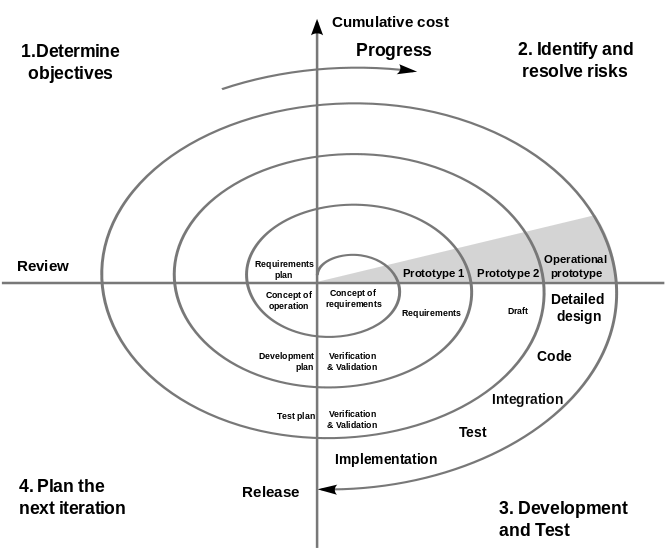
\includegraphics[width = 12cm]{./figures/spiral-model}\\
Figure 1: Spiral Development\\
\end{center}

For source management, our team will use GitHub which offers support for issue tracking, collaboration, and version management. Additionally, we will use GitHub's branching ability to manage the deployment and deployment of different stages of the source. Organization of the code will be along \verb|scopes|, meaning that the source's intention and ability will expand to a new, defined \verb|scope|. Contributions will be organized on a per-contributor branching scale.\\

Our team will use Trello for administrative task management such as deadlines, team updates, and communication about the state of the project. Trello provides a Kanban view of ``cards'' which will allow our team to organize tasks in different states.

\subsection{Experimental Methodology}
Our team will use a six-stage experimental methodology. This includes the initial development of the boilerplate to wrap the system, including the Jupyter Notebook and the various utility functions for downloading content and models. The methodology focuses on the same incremental attitude towards progress.

\begin{enumerate}
    \itemsep0em 
    \item Begin with writing a boilerplate to train models.
    \item Train a model for identifying the difference in car makes.
    \item Write a test framework to evaluate and provide stats on efficiency.
    \item Train a model for the vehicle identification.
    \item Run the experiment and gather results.
    \item Evaluate results.
\end{enumerate}

\section{Evaluation Methods}
\subsection{Development Evaluation}
To make sure our code is structured and unified we plan on using GitHub Actions workflow.\cite{githubWorkflows} GitHub Actions is a tool that help us create an automated process that will build and test our code. This will make testing of the code easier and quicker since we reduce the manual test burden. We plan on creating a workflow that is triggered when a developer pushes to the repository. The purpose of this workflow will be to lint the code. Since we code in Python we will use \textit{Pylint} and \textit{Flake8}.\cite{linting}\\

It is possible to have several workflows and they are highly configurable, but we will be starting of with only one. We prefer to start of small and create one effective, yet simple, workflow that will aid us in the development process. Spending to much time on workflows will simply not be worth it, since this project has a rather short time frame.

\subsection{AI System Evaluation}
\subsubsection{Qualitative Evaluation}
With the M.L. system, we expect to receive results in the raw format of object identification and tagging on a static image. However, this data can be further analyzed \textit{en masse} by applying statistical methods for how the model performed compared to the known state. For example, images with known military vehicles ranging from 1-10 can be fed through the system and the identification results analyzed in a spreadsheet and graphed. This will give both a visual identifier that the system was able/unable to identify the vehicles and a visual graph of the data collectively across tests.

\subsubsection{Quantitative Evaluation}
The M.L. system will provide quantitative results by providing statistical accuracy and probability measures for its ability to correctly identify a civilian or military vehicle. This will be conducted as a broad test with several tens or hundreds of test images. With the known value for civilian/military vehicles, standard equations can be applied using values such as:

\begin{itemize}
    \itemsep0em
    \item True Positive
    \item False Positive
    \item True Negative
    \item False Negative
\end{itemize}

By using these, the system can be evaluated for its performance and generate an accuracy value. This value can then be used as the range of the function of the M.L. system. The model and system can then be adjusted to improve this value, causing the function (M.L. system) to perform better.

\section{Limitations}
The M.L. system our team will develop has several clear limitations, both deterministic and indeterministic. The relevant variables that describe the limitations on the system are:

\begin{enumerate}
    \itemsep0em 
    \item The extent and variability in vehicles that the model is trained on, including the variability posed by regime changes and organic development.
    \item The implementation of the data source and its photographic clarity.
    \item The processing capabilities of the device on which the analysis is being conducted (i.e., the processing power available may significantly influence the confidence metric)
\end{enumerate}

The relevant limitations posed by this system are:
\begin{itemize}
    \itemsep0em 
    \item Additional infrastructure must be constructed in order to use the confidence metric as a variable in cost-value analysis when targeting human beings.
    \item Analysis and insight is limited by the training data provided, with clear analytical leaps when the vehicles cannot be referenced to vehicles in the data set
    \item Does not limit or eliminate the ability for adversaries to use civilian vehicles as a shield, requiring human interactions
    \item Both civilian and military vehicles have different designs around the world. It's likely that the data sets we use are heavily weighted towards the American, or other large nations, design of vehicles. We deem the work load of creating our own data set, with a more even distribution of vehicles from around the world, to be to high. Therefor accuracy results are likely to differ depending on the what nation the vehicle belongs to.
\end{itemize}

\bibliography{ref}

\end{document}
%%% Local Variables: 
%%% mode: latex
%%% TeX-master: t
%%% End: 

